\documentclass[a4paper, 11pt, twoside]{article}
\usepackage{amssymb}
\usepackage{amsmath}
\usepackage{listings}
\usepackage{pgfplots}
\usepackage{graphicx}
\begin{document}
\title{STAT6039 Assignment 2}
\author{Rui Qiu}
\date{2017-04-25}

\maketitle

\paragraph{Problem 1} A continuous random variable $Y$ has PDF (probability density function)

\[ 
f(y)=
\begin{cases}
	2e^{ky}, y>0\\
	\frac{1}{6}, -6<y<-3      
\end{cases}
\]

\paragraph{(a)} Determine the  value of the constant $k$. Then sketch the PDF. Finally, derive and sketch $Y$'s CDF (cumulative distribution function).

\paragraph{Solution:}

\[
\begin{split}
	\int^{-3}_{-6}\frac{1}{6}dy &= \frac{1}{6}y\bigg\rvert^{-3}_{-6}=\frac{1}{6}(-3+6)=\frac{1}{2}\\
	\int^\infty_{0}2e^{ky}dy&=\frac{2}{k}e^{ky}\bigg\rvert^{\infty}_0=\frac{2}{k}(e^{ky}-1)=1-\frac{1}{2}
\end{split}
\]

Observe that, only when $k<0$, $e^{ky}-1$ would converge. Otherwise, it would diverge to infinity. Therefore, $k=-4$, as

\[\lim_{y\to\infty}\frac{2}{k}(e^{ky}-1)=\frac{2}{k}(-1)=\frac12\]

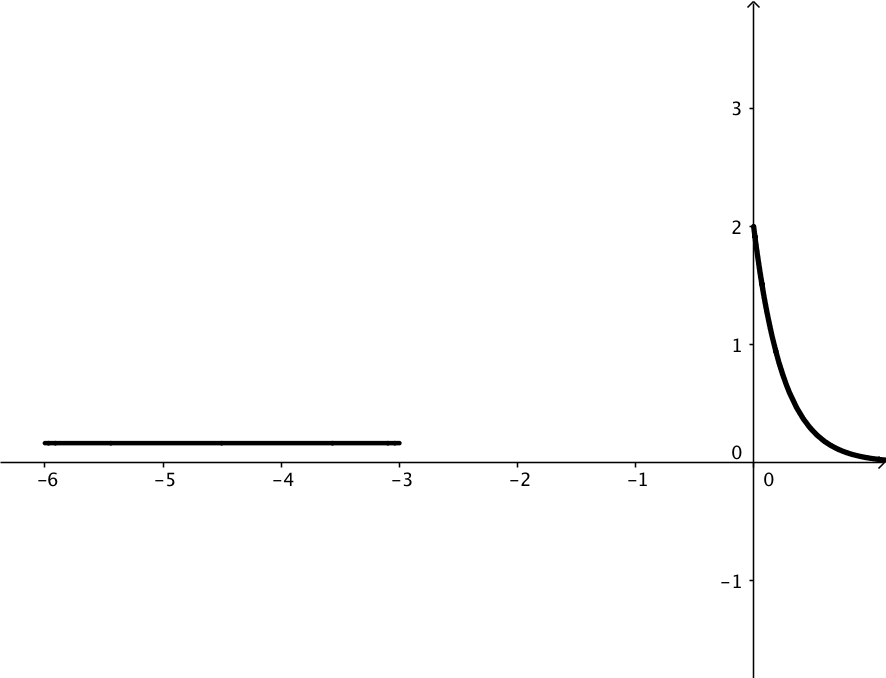
\includegraphics{image/1a-pdf}

Then we derive the CDF piece by piece:

For $-6<y<-3$,

\[\int^y_{-\infty}\frac{1}{6}dt=\frac{1}{6}t+b\bigg\rvert^y_{-\infty}\]

for some constant $b$.

Plug in $y=-6, \frac{1}{6}y+b=0$, so $b=1$. Therefore, the CDF in $(-6,-3)$ is $\frac{1}{6}y+1.$

Similarly, for $y>0$,

\[\int^y_{-\infty}2e^{-4}dt=-\frac12e^{-4t}+b'\bigg\rvert^y_{-\infty}\]

for some constant $b'$.

Again we plug in $y=0, -\frac{1}{2}e^{-4y}+b'=\frac{1}{2}$, and solve for $b'$, which is $b'=1$. Therefore, the CDF in $(0, \infty)$ is $-\frac{1}{2}e^{-4y}+1$.

Since CDF is constant in other partitions of $\mathbb{R}$ except $(-6, -3)\cup (0,\infty)$. We can write our final CDF as following:

\[
F(y)=
\begin{cases}
0, &y \leq -6\\
\frac{1}{6}y+1, &-6 < y < 3\\
\frac{1}{2}, &-3\leq y\leq 0\\
-\frac{1}{2}e^{-4y}+1, &y > 0
\end{cases}
\]

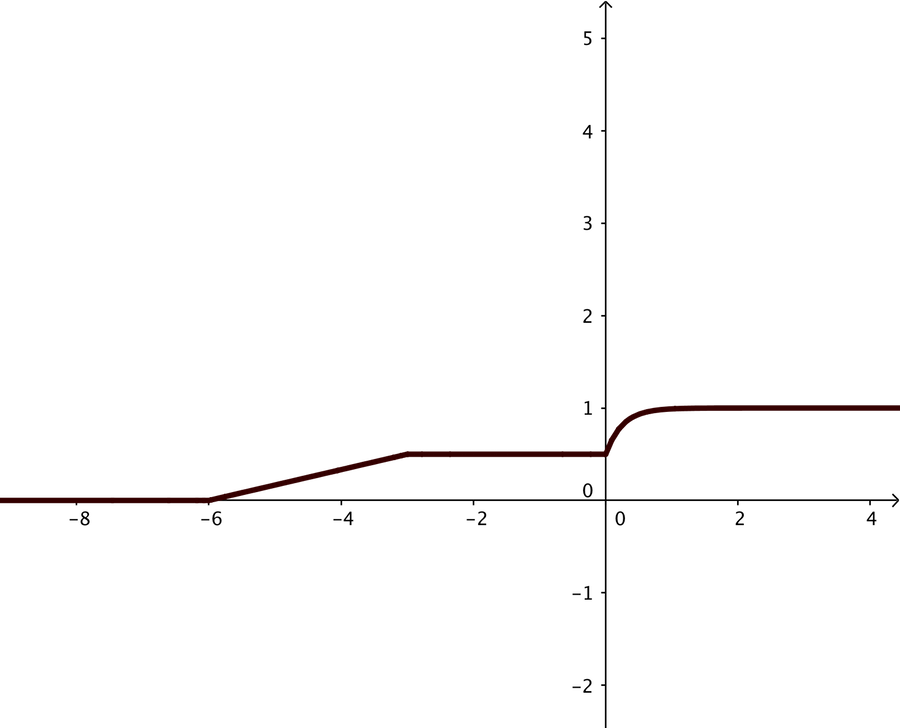
\includegraphics{image/1a-cdf}

\paragraph{(b)} Find $Y$'s mean, variance and standard deviation.

\paragraph{Solution:}

\[
\begin{split}
	E(Y)&=\int^{-3}_{-6}yf(y)dy + \int^{\infty}_0yf(y)dy\\
	&=\frac{1}{12}y^2\bigg\rvert^{-3}_{-6} + \frac{1}{2}y^2e^{-4y}+2y^2e^{-4y}\bigg\rvert^\infty_0\\
	&=\frac{1}{12}(9-36)+\left(-\frac{1}{8}e^{-4y}(4y+1)\right)\bigg\rvert^\infty_0\\
	&=-\frac{9}{4}+(0-(-\frac{1}{8}))\\
	&=-\frac{17}{8}\\
	\end{split}
\]

\[
\begin{split}
	E(Y^2)&=\int^{-3}_{-6}y^2\cdot \frac{1}{6}dy + \int^{\infty}_0y^2\cdot 2e^{-4y}dy\\
	&= \frac{1}{18}y^3\bigg\rvert^{-3}_{-6}+\left[-\frac{1}{16}e^{-4y}(8y^2+4y+1)\right]\bigg\rvert^\infty_0\\
	&=\frac{1}{18}[(-3)^3-(-6)^3]+\frac{1}{16}\\
	&=\frac{169}{16}
\end{split}
\]

\[
\begin{split}
	V(Y)&=E(Y^2)-[E(Y)]^2=\frac{169}{16}-\left(-\frac{17}{8}\right)^2=\frac{387}{64}\\
	\sigma_Y&=\sqrt{\frac{387}{64}}=\frac{3\sqrt{43}}{8}
\end{split}
\]

\paragraph{(c)} Find $Y$'s mode and median.

\paragraph{Solution:}

By definition, mode is the where the largest PDF exists, which is $y=0$.

And median is where $F(y)=\frac{1}{2}$. In this case, our median is not a single number, but a range from $-3\leq y\leq 0$.

\paragraph{Problem 2} A continuous random variable $Y$ has CDF

\[F(y)=
\begin{cases}
	a + \frac{ay}{2}, -2 < y < 0\\
	1-be^{-cy^3}, y > 0
\end{cases}
\]

\paragraph{(a)} Sketch the CDF when $a=\frac{1}{2}, b=\frac{1}{2}$ and $c=1$. Then derive $Y$'s pdf generally, and sketch it when $a=\frac{1}{2}, b=\frac{1}{2}$ and $c=1$. Finally, write down the range of possible values for $a,b$ and $c$.

\paragraph{Solution:} When $a=b=\frac12, c=1$,

\[F(y)=\begin{cases}\frac12 + \frac14y, &-2<y<0\\ 1-\frac12 e^{-y^3}, &y>0.\end{cases}\]

Then CDF is sketched as below:

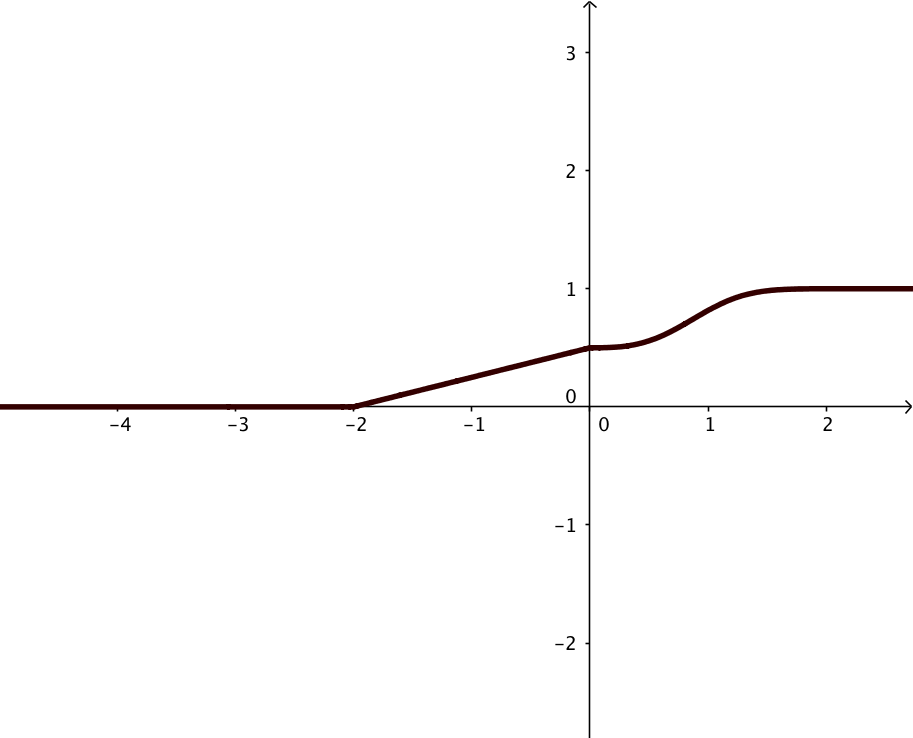
\includegraphics{image/2a-cdf}

For general PDF, we take the derivatives of piecewise CDF:

\[f(y)=\begin{cases}
	\frac{a}{2}, &-2<y<0\\
	3bcy^2e^{-cy^3}, &y>0
\end{cases}\]

And again, when $a=b=\frac{1}{2}, c=1$,

\[f(y)=\begin{cases}
	\frac{1}{4}, &-2<y<0\\
	\frac32y^2e^{-y^3}, &y>0
\end{cases}\]

So the PDF looks like:

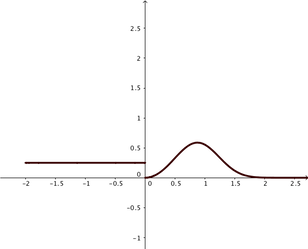
\includegraphics{image/2a-pdf}

Finally, about the the possible range of $a,b,c$.

\begin{enumerate}
	\item First we observe the CDF $F(y)$, when $y\rightarrow\infty$, $F(y)$ should converge to $1$, and $F(y) \leq 1$, so $b\geq 0$. (Otherwise, $F(y)>1$)
	\item Similar to Problem 1, only a non-positive $c$ can make $e^{-cy^3}$ converge. So $c\geq 0$.
	\item Consider this function continuous, so there should be no ``jump'' in the CDF. So the two pieces should meet at the same intersection ($y=0$ in this case), i.e. $a+\frac{a\cdot 0}{2} = 1-be^{-c\cdot 0^3}\implies a= 1-b$. Since $b\geq 0$, then $a\leq 1$.
	\item Also for $-2<y<0$, the CDF has $a+\frac{ay}{2}\geq 0$. So $a(2+y)\geq 0$, therefore $a\geq 0$ as $2+y > 0$ for $-2<y<0.$
	\item Back to the restriction $a=1-b$, so we have $0\leq 1-b \leq 1 \implies 0\leq b \leq 1.$
\end{enumerate}

Hence, $a\in [0,1], b\in [0, 1], c\in (0, \infty)$ when $b=0$ but $c\in\mathbb{R}$ when $b>0$. Also $a+b=1$.

\paragraph{(b)} Find $P(Y>-1|Y<1)$ when $a=\frac{1}{2}, b=\frac{1}{2}$ and $c=1$.

\paragraph{Solution:}

\[
\begin{split}
	P(Y>-1|Y<1)&=\frac{P(-1<Y<1)}{P(Y<1)}\\
	&=\frac{F(1)-F(-1)}{F(1)}\\
	&=\frac{1-\frac{1}{2}e^{-1}-\frac{1}{4}}{1-\frac{1}{2}e^{-1}}\\
	&=\frac{2-3e}{2-4e}\\
	&\simeq 0.69365
\end{split}
\]

\paragraph{Problem 3} A discrete random variable has PDF $p(y)=bk^y, y=0,1,2,\dots$

\paragraph{(a)} Sketch this PDF when $b=k=\frac{1}{2}$. Then derive $Y$'s CDF when $b=k=\frac{1}{2}$ and sketch it. Finally, write down the range of possible values for $b$ and $k$.

\paragraph{Solution:} For $b=k=\frac12$, 

\[f(y)=p(y)=\left(\frac12\right)^{y+1}, y=0,1,2,\dots\]

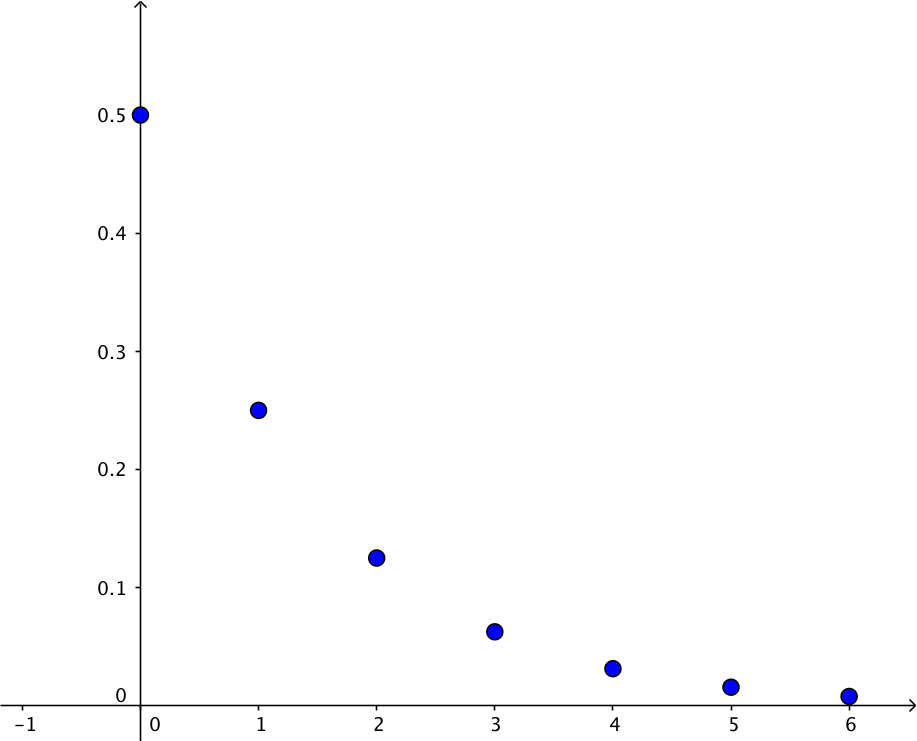
\includegraphics{image/3a-pdf}

\[F(y)=\begin{cases}
0,\ &y<0\\
\frac{1}{2},\ &0\leq y< 1\\
\frac{3}{4},\ &1\leq y<2\\
\frac{7}{8},\ &2\leq y<3\\
\frac{15}{16},\ &3\leq y<4\\
\frac{31}{32},\ &4\leq y<5\\
\dots &\dots	
\end{cases}
\]

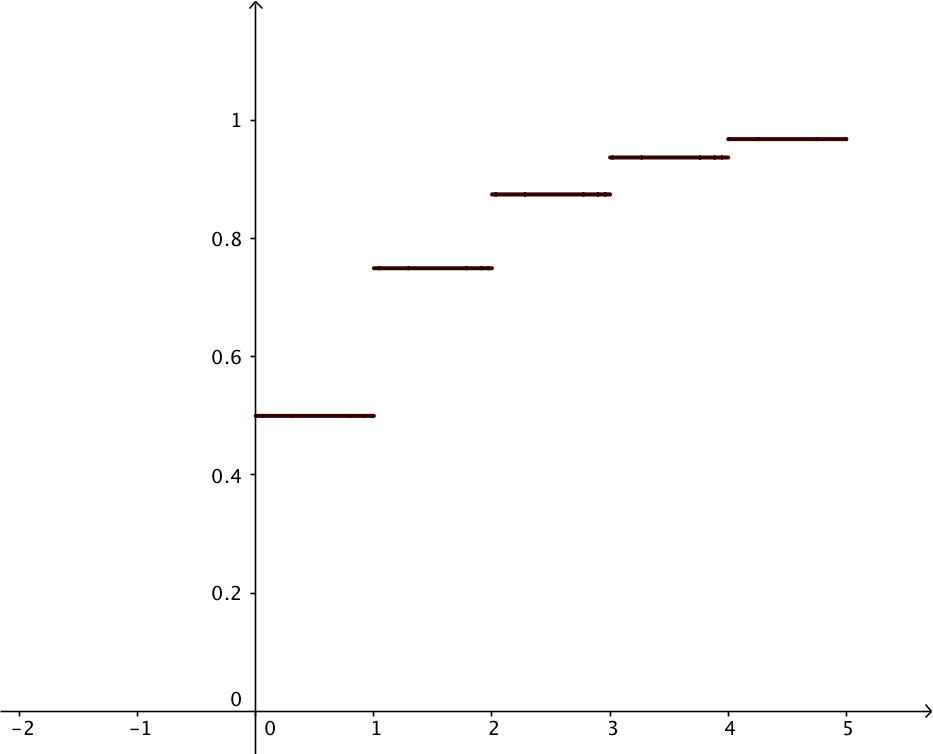
\includegraphics{image/3a-cdf}

\begin{itemize}
	\item Our requirement for $f(0)+f(1)+\cdots$ is that it finally converges to $1$. This is to test the convergence of series $\sum^{\infty}_{y=0}bk^y$.
	\item Note that, since no $f(i) > 1$ for any integer $i$, so the greatest $f(i)$ occurs when $i=0$, i.e. $0<f(0)=bk<1$. Otherwise, if $f(0)$ is not the greatest, that means for $y$ increases, the $f(y)$ increases, then the sum of $f(y)$'s would blow up, contradicting the fact that the series is convergent.
	\item Then we when our series is convergent. If our series is convergent, ratio test should hold, i.e. $\frac{f(y+1)}{f(y)}<1$, so $k<1\implies 0<k<1$ and $0<b<1$.
\end{itemize}

To conclude, the possible range for $k, b$ are both $(0,1)$.

\paragraph{(b)} Find $Y$'s mgf (moment generating function, $m(t)$ generally. Then sketch this mgf when $b=k=\frac{1}{2}$, showing the points at $t=0$ and $t=0.2$. Using the mgf method or otherwise, find the variance of $Y$ when $b=k=\frac{1}{2}$.

\paragraph{Solution:} 

\[\begin{split}
	m(t)&=E(e^{Yt})=\sum^\infty_{y=0}e^{bk^yt}\cdot bk^y\\
	&=\frac{b}{1-e^tk}
\end{split}
\]

When $b=k=\frac{1}{2}$, the general MGF is: 

\[m(t)=\frac{1}{2-e^t}\]

Note that $m(t)$ is undefined when $t>\log{2}$.

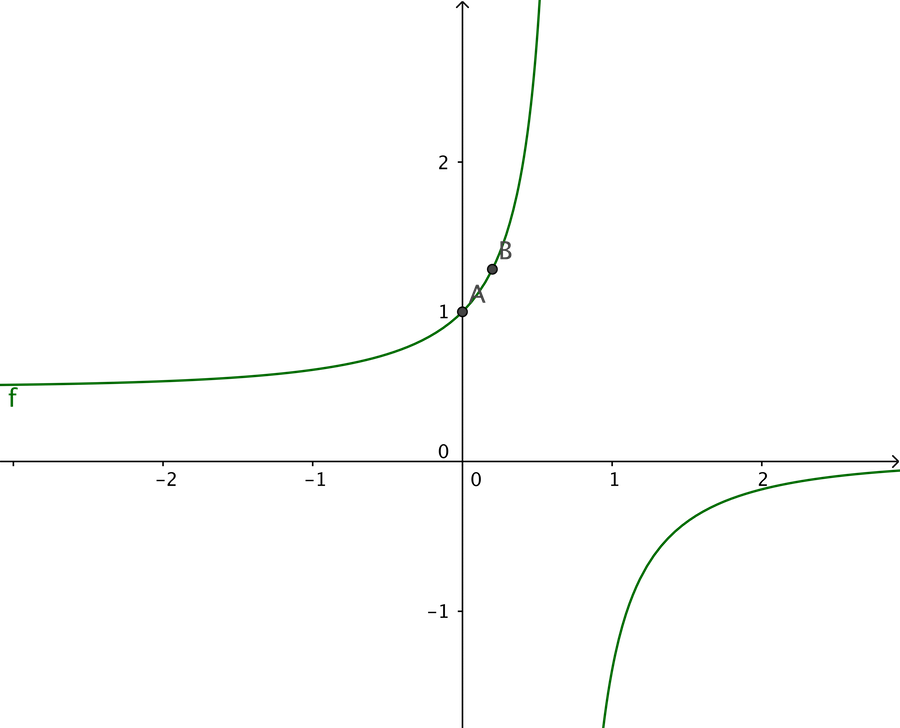
\includegraphics{image/3b-mgf}

The graph of MGF is shown above, and point $A$ represents $m(0)$, and point $B$ represents $m(0.2)$.\\

\[
\begin{split}
	E(Y)&=\mu=m'(0)=\frac{e^0}{(2-e^0)^2}\\
	&= 1\\
	E(Y^2)&=m''(0)=\frac{e^0(2-e^0)^2+2e^{2\cdot 0}(2-e^0)}{(2-e^0)^4}\\
	&=3\\
	V(Y)&=E(Y^2)-[E(Y)]^2\\
	&=3-1^2\\
	&=2
\end{split}
\]

\paragraph{Problem 4} In a certain country, the weights of female adults (ages 18 and up) are approximately normally distributed. About one fifth of the female adult population is heavier than 91kg, and one quarter is lighter than 46kg.

\paragraph{(a)} Find the proportion of female adults in the country who are heavier than 60kg.

\paragraph{Solution:} Suppose the weights of female adults is a random variable $Y\sim N(\mu, \sigma)$. We now have $P(Y>91)=0.2, P(Y<46)=0.25$.

Since 

\[Z=\frac{Y-\mu}{\sigma}\sim N(0,1)\]

Then 

$P(Z > z_1)=0.2 \implies P(Z<z_1)=0.8$

$P(Z < z_2)=0.25$

Check z-table we have

\[
\begin{split}
	z_1&=\frac{91-\mu}{\sigma}=0.84\\
	z_2&=\frac{46-\mu}{\sigma}=-0.675	
\end{split}
\]

Solve for both $\mu, \sigma$ we get $\mu=66.0495$kg, $\sigma=29.7030$kg.

Therefore, 

\[P(Y>60)= 1- P(Z < \frac{60-\mu}{\sigma})\approx 1-P(Z<-0.2037)= 1- 0.4207=0.5793\]

So the proportion of female adults in the country who are heavier than 60kg is about 57.93\%.

\paragraph{(b)} A female adult, Lisa, has been randomly chosen from the population of the country. We are told that her weight is below average. Find the probability that Lisa weighs more than 60kg.

\[
\begin{split}
	P(60<Y<\mu)&=P(Y<\mu)-P(Y<60)=0.5-0.4207=0.0793\\
	P(Y>60|Y<\mu)&=\frac{P(60<Y<\mu)}{P(Y<\mu)}=\frac{0.0793}{0.5}=0.1586
\end{split}
\]

Therefore, the probability that Lisa weighs more than 60kg is 0.1586.

\paragraph{Problem 5} A straight wooden plank of length 2m has been purchased for \$34. This plank is about to be sawed into two at a point chosen randomly along it. Each of the two resulting short planks will be sawed \textbf{\textit{lengthwise}} into twelve identical sticks. Next, two perfectly cubic frames will be constructed from the twenty four sticks. Then both frames will be made into huge dice by covering them, each on all six sides, with a type of red plastic sheet which costs \$42 per square metre. Next, each die will be filled with a bouncy rubber material which costs \$66 per cubic metre. Finally, the usual number of dots will be put onto the dice. For each die whose total surface area is at least 5400 square centimetres, the dots will be made of gold at a cost of \$15 each; for each die smaller than this, the dots will be painted on with black paint at negligible cost.

For how many dollars should the two dice be sold (in advance) so that the expected profit is \$700?

\paragraph{Solution:} Clearly, we have:

\[E(\text{Price})-E(\text{Cost})=E(\text{Profit})\]

Suppose the two separated parts of plank have length $X$ and $2-X$ (in metres), and $X\sim U(0,2)$. And we also do some unit conversion ahead: $5400\text{cm}^3\implies 900\text{cm}^2$ per face $\implies$ each length is at least $0.3$m.

Then the expected cost is

\[
\begin{split}
	\text{Cost except dots}&=34+\left[\left(x\right)^2\cdot 6+\left(2-x\right)^2\cdot 6\right]\cdot 42\\
	&+\left[\left(x\right)^3+\left(2-x\right)^3\right]\cdot 66\\
	&=900x^2-1800x+1570
\end{split}
\]

Since $X\sim U(0,2)$,

\[\begin{split}
	E(X)&=\frac{1}{2-0}\int^2_0xdx = \frac{1}{4}x^2\bigg\rvert^2_0=1\\
	E(X^2)&=\frac{1}{2-0}\int^2_0x^2dx = \frac{1}{6}x^3\bigg\rvert^2_0=\frac{4}{3}
\end{split}
\]

Then

\[E(\text{Cost except dots})=900\cdot \frac{4}{3} - 1800\cdot 1 + 1570=970\]

Also, the expected ``dots cost'' is:

\[
\begin{split}
	E(\text{Dots cost})&= P(x>0.3)\cdot 21\cdot 15 + P(2-x>0.3)\cdot 21\cdot 15\\
	&= \frac{2-0.3}{2}\cdot 21\cdot 15 + \frac{1.7}{2}\cdot 21\cdot 15\\
	&= 535.5
\end{split}
\]

Hence,

\[\begin{split}E(\text{Price}) &= E(\text{Cost except dots}) + E(\text{Dots cost}) + E(\text{Profit})\\&=970+535.5+700\\&=\$2205.5\end{split}\]	

The two dice should be sold at \$2205.5 for an expected \$700 profit. 

\end{document}